\subsection{Abbildungen}
\begin{figure}[h]
	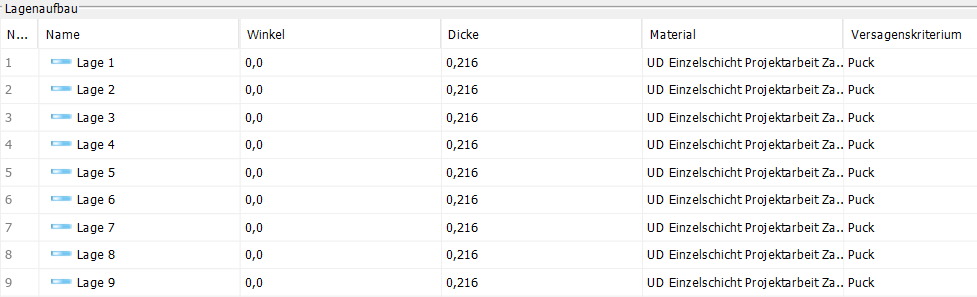
\includegraphics[width=1.0\textwidth]{Bilder/Lagenaufbau Holmgurte.png}
	\caption{Lagenaufbau Holmgurte}
	\label{fig:Lagenaufbau Holmgurte}
\end{figure}
\begin{figure}
	\includegraphics[width=1.0\textwidth]{Bilder/Lagenaufbau Steg dünn.png}
	\caption{Lagenaufbau Steg Bereich $III$}
	\label{fig:Lagenaufbau Steg dünn}
\end{figure}
\begin{figure}
	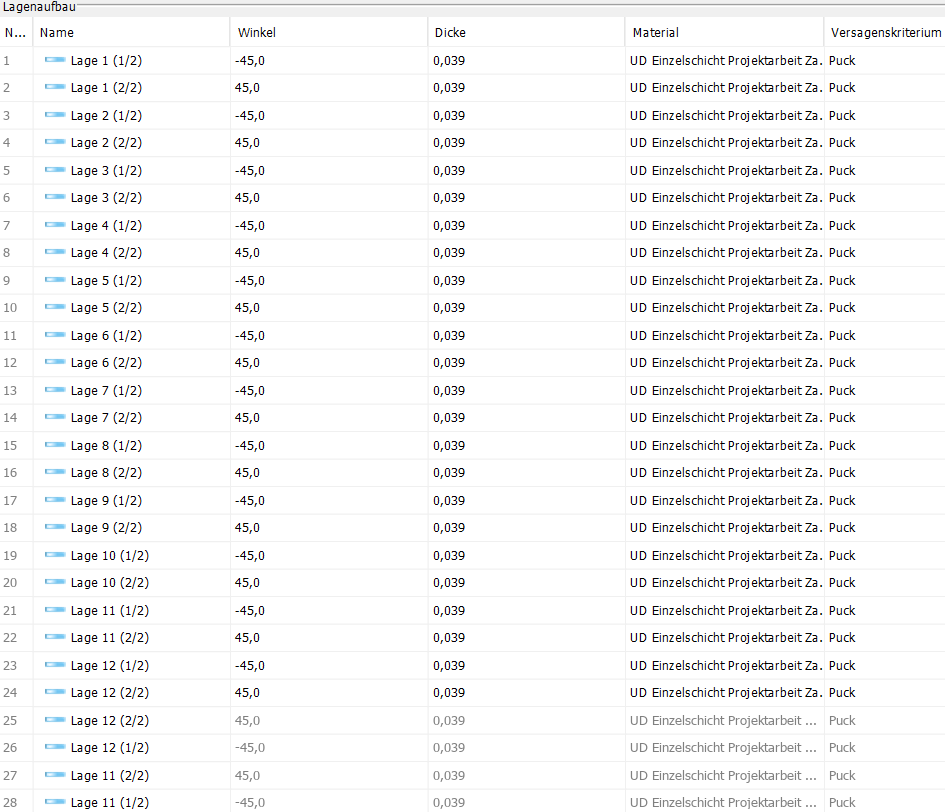
\includegraphics[width=1.0\textwidth]{Bilder/Lagenaufbau Steg dick.png}
	\caption{Lagenaufbau Steg Bereich $I$\&$II$}
	\label{fig:Lagenaufbau Steg dick}
\end{figure}
\begin{figure}
	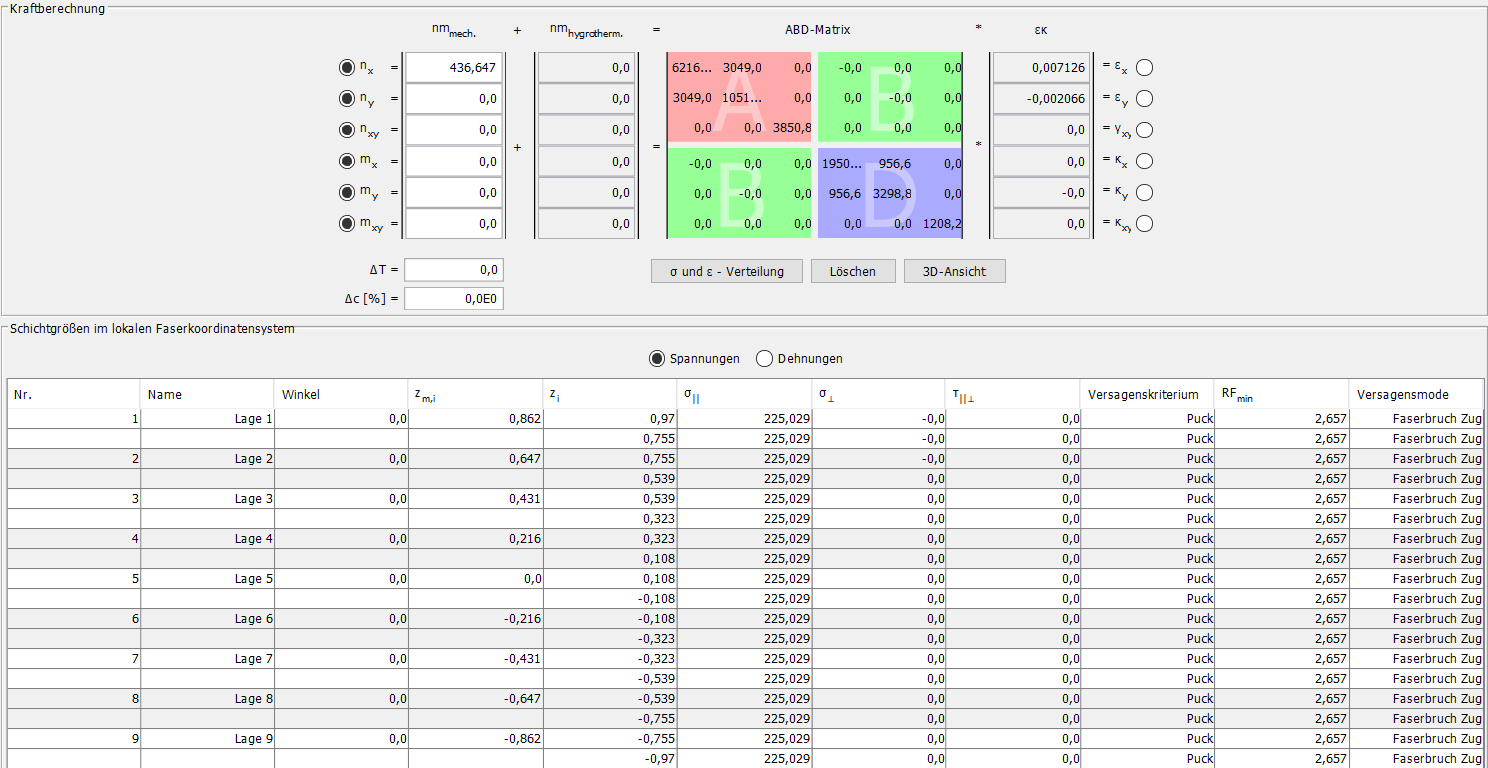
\includegraphics[width=1.0\textwidth]{Bilder/Berechnung Holmgurte.png}
	\caption{Berechnung Holmgurte}
	\label{fig:Berechnung Holmgurte}
\end{figure}
\begin{figure}
	\includegraphics[width=1.0\textwidth]{Bilder/Berechnung Steg dünn.png}
	\caption{Berechnung Steg Bereich $III$}
	\label{fig:Berechnung Steg dünn}
\end{figure}
\begin{figure}
	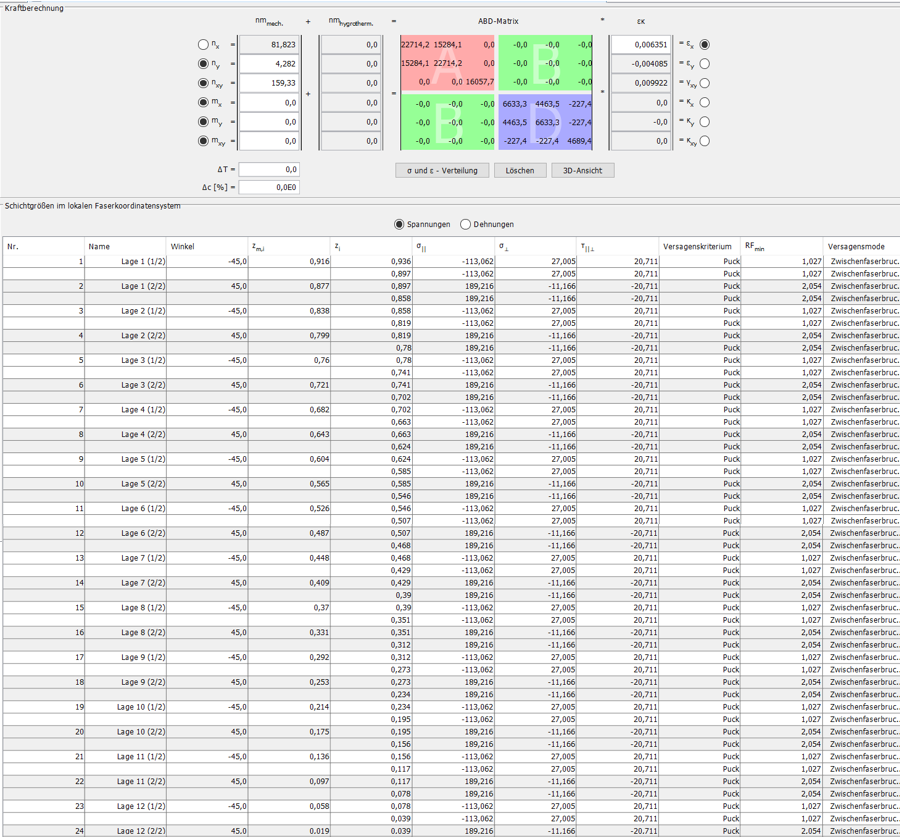
\includegraphics[width=1.0\textwidth]{Bilder/Berechnung Steg dick.png}
	\caption{Berechnung Steg Bereich $I$\&$II$}
	\label{fig:Berechung Steg dick}
\end{figure}
\begin{figure}
	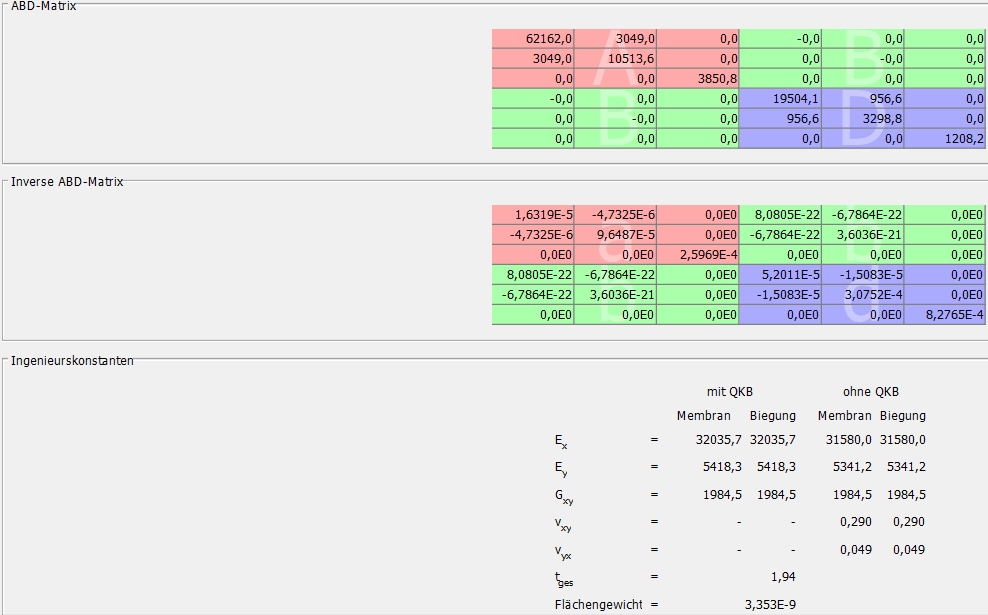
\includegraphics[width=1.0\textwidth]{Bilder/Konstanten Holmgurte.png}
	\caption{Ingenieurskonstanten Holmgurte}
	\label{fig:Ingenieurskonstanten Holmgurte}
\end{figure}
\begin{figure}
	\includegraphics[width=1.0\textwidth]{Bilder/Konstanten Steg dünn.png}
	\caption{BerechnIngenieurskonstantenung Steg Bereich $III$}
	\label{fig:Ingenieurskonstanten Steg dünn}
\end{figure}
\begin{figure}
	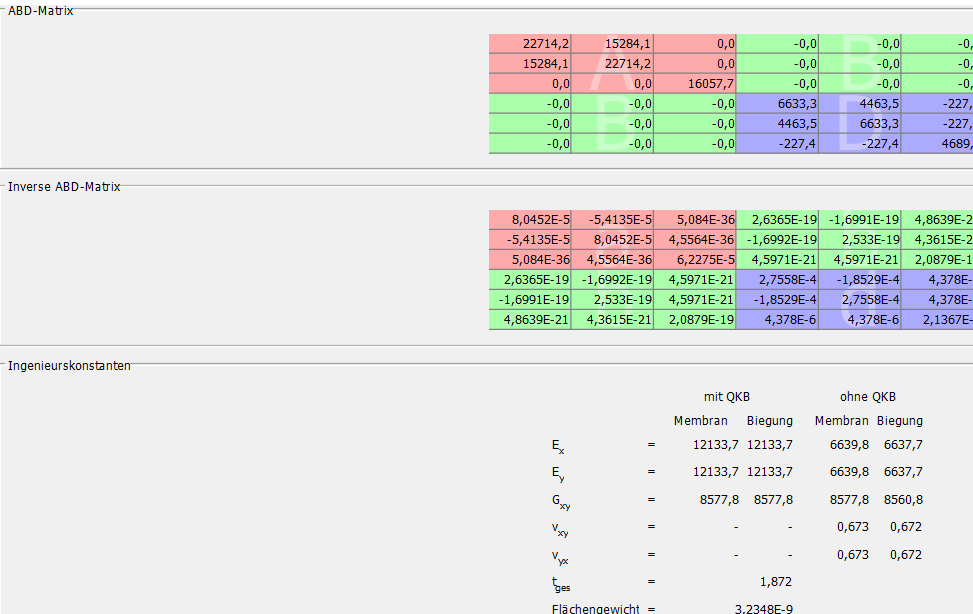
\includegraphics[width=1.0\textwidth]{Bilder/Konstanten Steg dick.png}
	\caption{Ingenieurskonstanten Steg Bereich $I$\&$II$}
	\label{fig:Ingenieurskonstanten Steg dick}
\end{figure}
